\documentclass[conference]{IEEEtran}
\IEEEoverridecommandlockouts
% The preceding line is only needed to identify funding in the first footnote. If that is unneeded, please comment it out.
%Template version as of 6/27/2024

\usepackage{cite}
\usepackage{amsmath,amssymb,amsfonts}
\usepackage{algorithmic}
\usepackage{graphicx}
\usepackage{textcomp}
\usepackage{xcolor}
\def\BibTeX{{\rm B\kern-.05em{\sc i\kern-.025em b}\kern-.08em
    T\kern-.1667em\lower.7ex\hbox{E}\kern-.125emX}}
\begin{document}

\title{INS 3D Reduced Inertial Sensor Mechanization}

\author{\IEEEauthorblockN{Mazen Elaraby}
\IEEEauthorblockA{\textit{Department of Electrical and Computer Engineering} \\
\textit{Queen's University}\\
Kingston, Canada 
}}

\maketitle

\begin{abstract}
Reliable and cost-effective navigation systems play a critical role in modern applications such as autonomous vehicles, drones, and mobile robots, where continuous position estimation is essential for safe and efficient operation. Inertial Navigation Systems (INS) provide robust navigation capabilities independent of external signals, avoiding issues like GPS jamming, spoofing, and environmental occlusion. However, deploying a full Inertial Measurement Unit (IMU) remains costly due to the reliance on multiple gyroscopes, making it impractical for low-cost robotic and vehicular platforms. Recent efforts have focused on reducing sensor requirements through gyro-free or reduced-sensor IMU configurations. This paper builds upon the Reduced Inertial Sensor System (RISS), which uses three accelerometers, an odometer, and a single gyroscope to address errors associated with uncompensated gyroscopic biases. We propose enhancements to the RISS approach by incorporating heuristic-based methods to mitigate noise and error accumulation, including stopping mechanization during vehicle stationarity and applying filtering techniques for improved pitch and roll estimation. These improvements enhance navigation accuracy while maintaining cost efficiency, making the solution viable for low-cost autonomous systems.
\end{abstract}

\begin{IEEEkeywords}
Land Vehicle navigation, Inertial Navigation System, Reduced Inertial Sensor System.
\end{IEEEkeywords}

\section{Introduction}
Accurate and reliable navigation solutions are critical across a wide range of applications, including robotics, ground vehicles, drones, and autonomous systems. As these technologies continue to advance, the demand for robust navigation systems has surged, driven by the need for precision in environments where global positioning and external signals may be unreliable or unavailable. Autonomous vehicles, for instance, require real-time navigation to maintain safety and efficiency in both structured and unstructured terrains. Similarly, drones and mobile robots rely on continuous position and orientation information to execute tasks such as surveillance, mapping, and transportation.

Inertial Navigation Systems (INS) offer significant advantages in these contexts. Unlike external sensor-based navigation solutions such as GPS, an INS does not depend on external signals, making it immune to vulnerabilities such as jamming, spoofing, and multipath interference. While techniques like LiDAR, radar, and visual odometry provide valuable navigation data, they are susceptible to environmental factors such as low visibility, surface reflectivity, and signal occlusion. These limitations have prompted research to explore the development of more robust and self-contained navigation solutions.

Despite considerable advancements in Microelectromechanical Systems (MEMS) technology, deploying a full Inertial Measurement Unit (IMU) remains expensive, particularly for low-cost vehicles and robotic platforms. A complete IMU typically comprises three accelerometers and three gyroscopes, with gyroscopes often being the most costly and sensitive component. To address these challenges, research has increasingly focused on reducing the number of sensors in IMUs to lower costs while maintaining acceptable navigation performance. One approach even involves the development of gyro-free inertial measurement units (GF-IMU), which aim to eliminate or minimize the use of gyroscopes.

Building on this trend, the Reduced Inertial Sensor System (RISS) proposed in  \cite{noureldin2013} demonstrated an alternative configuration that reduces sensor requirements. RISS utilizes three accelerometers, an odometer, and a single gyroscope, effectively eliminating errors that arise from uncompensated biases in horizontal gyroscopes. This configuration has shown potential in providing cost-effective and reliable navigation, especially in resource-constrained applications.

This paper extends the RISS methodology by implementing additional heuristic-based techniques to further mitigate its limitations. Specifically, mechanisms are introduced to halt the navigation system during stationary periods, preventing the accumulation of errors. Additionally, filtering strategies are applied to reduce noise in the estimation of pitch and roll, which are computed using accelerometer data. These enhancements aim to improve the overall accuracy and robustness of the reduced-sensor INS solution, making it more viable for deployment in low-cost autonomous systems.

\section{Implementation Details}

\subsection{3D RISS Mechanization}\label{AA}

The 3D Reduced Inertial Sensor System (RISS) is configured as shown in Figure~\ref{fig:setup}. The system includes a single-axis gyroscope, with its sensitive axis aligned along the vertical direction of the vehicle, three orthogonal accelerometers, and an odometer. The gyroscope provides measurements of the rotation rate in the body frame, while the accelerometers measure the linear acceleration along their respective axes. The odometer measures the forward speed of the vehicle.

\begin{figure}[htbp]
\centerline{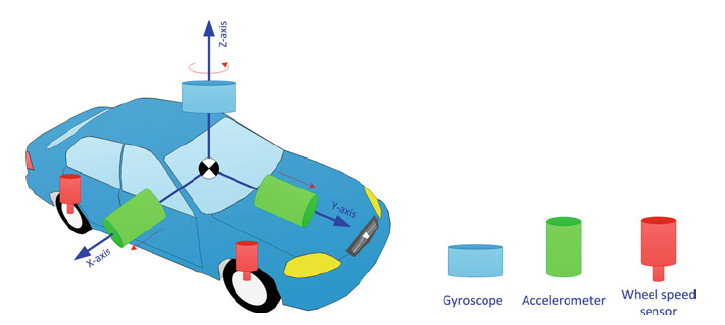
\includegraphics[width=0.48\textwidth]{plots/setup.png}}
\caption{3D RISS Sensor Setup.}
\label{fig:setup}
\end{figure}

The gyroscope measures the rotation rate in the body frame, which needs to be transformed to the local-level frame (LLF) while taking into consideration two main factors. The first is the component of Earth’s rotation along the vertical direction, given by \( \omega_e \sin \varphi \), where \( \omega_e \) is the Earth’s rotation rate and \( \varphi \) is the latitude. The second factor is the change in the orientation of the local-level frame with respect to the Earth, determined by the eastward velocity \( V_e \), altitude \( h \), and the normal radius \( R_N \). The rate of change of the yaw angle \( \dot{\gamma} \) is expressed as:
\begin{equation}
\dot{\gamma} = \omega_z - \omega_e \sin \varphi - \frac{V_e \tan \varphi}{R_N + h}
\label{eq:yaw}
\end{equation}


The pitch \( p \) and roll \( r \) angles are estimated using the readings of the three orthogonal accelerometers. The accelerometer readings along the three axes are denoted by \( f_x \), \( f_y \), and \( f_z \), while \( v_{od} \) is the forward speed measured by the odometer, and \( a_{od} \) is the forward acceleration obtained by differentiating the odometer’s speed measurements. The following equations are used for estimation:

\begin{equation}
r = \tan^{-1} \left( \frac{-(f_x + v_{od} \, \omega_z)}{f_z} \right)
\label{eq:roll}
\end{equation}

\begin{equation}
p = \tan^{-1} \left( \frac{-(f_y - a_{od})}{\sqrt{f_x^2 + f_z^2}} \right)
\label{eq:pitch}
\end{equation}


The odometer measures the forward velocity of the vehicle, which is aligned along the vehicle’s forward axis. To express this velocity in terms of the local-level frame axes (east \( V^e \), north \( V^n \), and up \( V^u \)), the following transformation is used:

\begin{equation}
\begin{pmatrix}
V^e \\
V^n \\
V^u
\end{pmatrix}
=
\begin{pmatrix}
-\sin \gamma \cos p \, v_{od} \\
\cos \gamma \cos p \, v_{od} \\
\sin p \, v_{od}
\end{pmatrix}
\label{eq:velocity_transform}
\end{equation}


where \( \gamma \) and \( p \) represent the yaw and pitch angles, respectively.

To obtain the geodetic position components, the velocity components in the local-level frame are transformed into geodetic coordinates. The velocity components are integrated over the sampling interval to compute the changes in latitude \( \varphi \), longitude \( \lambda \), and altitude \( h \) using the following transformation:

\begin{equation}
\begin{pmatrix}
\dot{\varphi} \\
\dot{\lambda} \\
\dot{h}
\end{pmatrix}
=
\begin{pmatrix}
0 & \frac{1}{R_M + h} & 0 \\
\frac{1}{(R_N + h) \cos \varphi} & 0 & 0 \\
0 & 0 & 1
\end{pmatrix}
\begin{pmatrix}
V^e \\
V^n \\
V^u
\end{pmatrix}
\label{eq:geodetic_transform}
\end{equation}


where \( R_M \) represents the meridian radius of curvature at a given latitude \( \phi \).

\begin{figure}[htbp]
\centerline{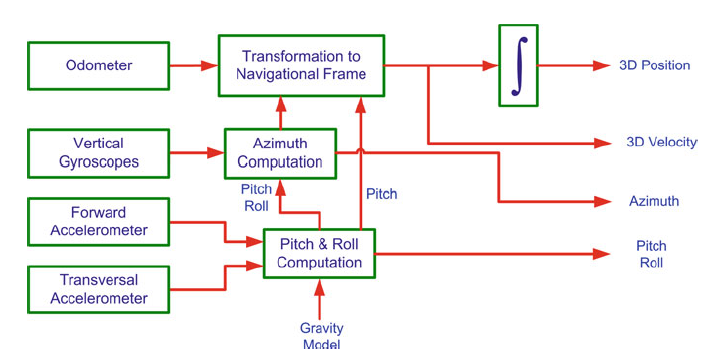
\includegraphics[width=0.48\textwidth]{plots/BD.png}}
\caption{A block diagram of the 3D RISS model.}
\label{fig:mechanization}
\end{figure}

The complete process of mechanization, including sensor inputs, coordinate transformations, and position estimation, is summarized in the block diagram shown in Figure~\ref{fig:mechanization}. The diagram illustrates how sensor measurements are processed sequentially to obtain accurate position estimates.

\subsection{Bias Estimation}
Estimating the bias of the gyroscope and accelerometers is crucial because even small sensor biases can accumulate over time, leading to significant errors in position, orientation, and velocity estimates. By accurately modeling and compensating for these biases, the overall navigation accuracy and system reliability are greatly improved, particularly in long-duration applications.

When the vehicle is stationary the accelerometers measure components due to gravity owing to the tilt from the horizontal plane by the pitch and roll angles. The accelerometer measurements are

\begin{equation}
\begin{pmatrix}
f_x \\
f_y \\
f_z
\end{pmatrix}
= R^b_\ell
\begin{pmatrix}
0 \\
0 \\
-g
\end{pmatrix}
= \left( R^\ell_b \right)^{T}
\begin{pmatrix}
0 \\
0 \\
-g
\end{pmatrix}
=
\begin{pmatrix}
g \cos p \sin r \\
-g \sin p \\
-g \cos p \cos r
\end{pmatrix}
\label{eq:gravity_projection}
\end{equation}

Therefore the accelerometer biases can be computed as
\begin{equation}
b_x = f_x - \cos(p) \sin(r) g
\label{eq:bias_x}
\end{equation}

\begin{equation}
b_y = f_y + \sin(p) g
\label{eq:bias_y}
\end{equation}

\begin{equation}
b_z = f_z + \cos(p) \cos(r) g
\label{eq:bias_z}
\end{equation}

As for the gyroscope, the bias term can be estimated by removing the stationary component from the measurements while the vehicle is stationary

\begin{equation}
b_w = \omega_z - \omega_e \sin(\varphi)
\label{eq:bias_gyro}
\end{equation}

\subsection{Mitigating Noise in Off-Plane Motion Estimation}

In 3D RISS mechanization, the estimation of off-plane motion, specifically the pitch \( p \) and roll \( r \) angles, relies on the readings of the three accelerometers. This technique effectively eliminates the need for horizontal gyroscopes, avoiding drift and the accumulation of uncompensated biases typically associated with these gyroscopes. However, the resulting pitch and roll estimates are prone to significant noise. The primary sources of this noise include the low sampling rate of odometer measurements and the inherent noise amplification introduced by the differentiation operation used to compute the forward acceleration \( a_{od} \) from the odometer’s speed measurement \( v_{od} \).

In signal processing terms, differentiation is mathematically equivalent to applying a high-pass filter. Given a continuous signal \( v_{od}(t) \), its derivative \( a_{od}(t) = \frac{d}{dt}v_{od}(t) \) emphasizes rapid changes in the signal. Mathematically, differentiation in the time domain corresponds to multiplication by \( j\omega \) in the frequency domain, where \( \omega \) is the angular frequency. This operation effectively amplifies high-frequency components, as shown in the transfer function of the differentiation operator:

\[
A(j\omega) = j\omega V(j\omega)
\]

Here, \( V(j\omega) \) is the Fourier transform of the speed signal \( v_{od}(t) \), and \( A(j\omega) \) is the Fourier transform of the acceleration signal \( a_{od}(t) \). The linear dependency on \( \omega \) implies that as frequency increases, the magnitude of the high-frequency components is amplified, which introduces noise when real-world signals are differentiated.

Since the estimation of pitch \( p \) and roll \( r \) directly relies on \( a_{od} \), any high-frequency noise present in the differentiation process propagates into the pitch and roll estimates. As a result, these estimates become unstable and noisy. This noise further propagates to the calculation of the upwards velocity \( V^u \), which depends on pitch and roll angles. Given that altitude \( h \) is obtained by integrating the vertical velocity over time, any noise in \( V^u \) accumulates, leading to large errors and instability in altitude measurements.
 
In this work, an alternative numerical differentiation technique has been employed along with low-pass filtering of the acceleration measurements. The selection of these methods was guided by the following key considerations: 
 
\begin{itemize}
    \item \textbf{Causal Structure:} Since the system operates in real-time, it can only access current and past measurements. Therefore, a filter with a causal structure is required.
    
    \item \textbf{Lag vs. Noise Suppression:} Filter hyperparameters were carefully selected to balance the smoothing of noisy acceleration estimates without introducing significant lag.
    
    \item \textbf{Computational Complexity:} Given the real-time requirements of the system, filters with low computational complexity were chosen. Additionally, filters with structures that are well-suited for hardware acceleration, such as vector/SIMD processors and FPGAs, were prioritized.
\end{itemize}

Here are the solutions studied:

\subsubsection{\textbf{Tustin's Approximation of the Derivative}}

The Tustin approximation provides a more stable and noise-resistant alternative to standard backward differentiation in discrete-time systems \cite{ogata2010}. By combining current and previous samples with adjustable weighting, it offers a balance between noise suppression and responsiveness, making it well-suited for noisy sensor signals. The approximation is given by:

\begin{equation}
\frac{dx}{dt} \approx \frac{2}{\Delta t} \cdot \frac{x[i] - x[i-1]}{1 + \beta}
\label{eq:tustin_approximation}
\end{equation}

Higher $\beta$ makes the derivative more responsive to current changes but sensitive to noise, while lower  $\beta$ smooths the derivative by giving more weight to past values, improving stability.

\subsubsection{\textbf{Moving Average Filter}}

The moving average filter is a simple yet effective technique for reducing high-frequency noise in signals by averaging a set of consecutive samples over a specified window. It is particularly useful when dealing with noisy measurements, as it smooths fluctuations without requiring complex computations. The moving average filter is defined by:

\begin{equation}
y[i] = \frac{1}{N} \sum_{k=0}^{N-1} x[i - k]
\label{eq:moving_average}
\end{equation}

The window size \( N \) controls the degree of smoothing applied by the filter. A larger \( N \) averages more samples, providing greater noise reduction but introducing a delay and potentially blurring rapid changes in the signal. A smaller \( N \) preserves fast signal variations but provides less noise suppression. Proper selection of \( N \) is crucial for balancing noise reduction and responsiveness in practical applications.

\subsubsection{\textbf{Exponential Moving Average Filter}}

Exponential smoothing, also known as the exponential moving average (EMA), is a common technique for smoothing time series data using an exponential weighting function. Unlike the simple moving average, which assigns equal weights to past observations, the EMA applies exponentially decreasing weights, giving more significance to recent data while gradually reducing the influence of older observations. The simplest form of exponential smoothing is given by:

\begin{equation}
y[i] = \alpha x[i] + (1 - \alpha) y[i - 1]
\label{eq:ema}
\end{equation}

The parameter \( \alpha \) controls the weighting of recent versus past samples. A larger \( \alpha \) places more weight on the current sample, making the filter more responsive to sudden changes but less effective at noise suppression. A smaller \( \alpha \) gives more weight to past values, providing greater smoothing and noise reduction at the cost of slower responsiveness. Proper tuning of \( \alpha \) ensures the right trade-off between noise reduction and adaptability.

\subsubsection{\textbf{Butterworth Low-Pass Filter}}

The Butterworth low-pass filter is a signal processing technique designed to attenuate high-frequency noise while preserving the essential low-frequency components of the signal. It is known for its maximally flat frequency response in the passband, making it ideal for applications where smooth and distortion-free filtering is critical \cite{manolakis2011}. The Butterworth filter is typically implemented as an IIR (Infinite Impulse Response) filter, and its general form in discrete time is:

\begin{equation}
y[i] = \sum_{k=0}^{N} b_k x[i-k] - \sum_{k=1}^{N} a_k y[i-k]
\label{eq:butterworth}
\end{equation}

The order of the Butterworth filter determines the sharpness of the frequency cutoff. A higher-order filter provides a steeper transition between the passband and stopband, allowing for more effective noise suppression. However, increasing the order may introduce more phase lag and computational complexity. Proper selection of the filter order balances noise reduction and signal fidelity, ensuring minimal distortion of the underlying data.

Table~\ref{table:complexity} summarizes the computational complexity of the discussed filters, presenting the exact number of multiplications and additions, as well as their asymptotic complexity using Big-O notation.


\begin{table}[htbp]
\caption{Computational Complexity of Filters}
\begin{center}
\begin{tabular}{|c|c|c|c|}
\hline
\textbf{Filter Type} & \textbf{Multiplications} & \textbf{Additions} & \textbf{Big-O Notation} \\ \hline
\textbf{Nth-order BW} & $2N + 1$ & $2N$ & $O(N)$ \\ \hline
\textbf{MA} & $N$ & $N - 1$ & $O(N)$ \\ \hline
\textbf{EMA} & $2$ & $1$ & $O(1)$ \\ \hline
\end{tabular}
\label{table:complexity}
\end{center}
\end{table}

\section{Results}

The system was tested using data collected from a single trajectory, covering approximately 12.6 km over a duration of 42 minutes. Two IMU units were employed for data collection: a high-end tactical IMU (HG1700, Honeywell) and a low-cost, automotive-grade MEMS-based IMU (VTI IMU). The speed readings have been obtained through the On-Board Diagnostics version II (OBD II) interface using a device called CarChip.

\begin{figure*}[htbp]
    \centering
    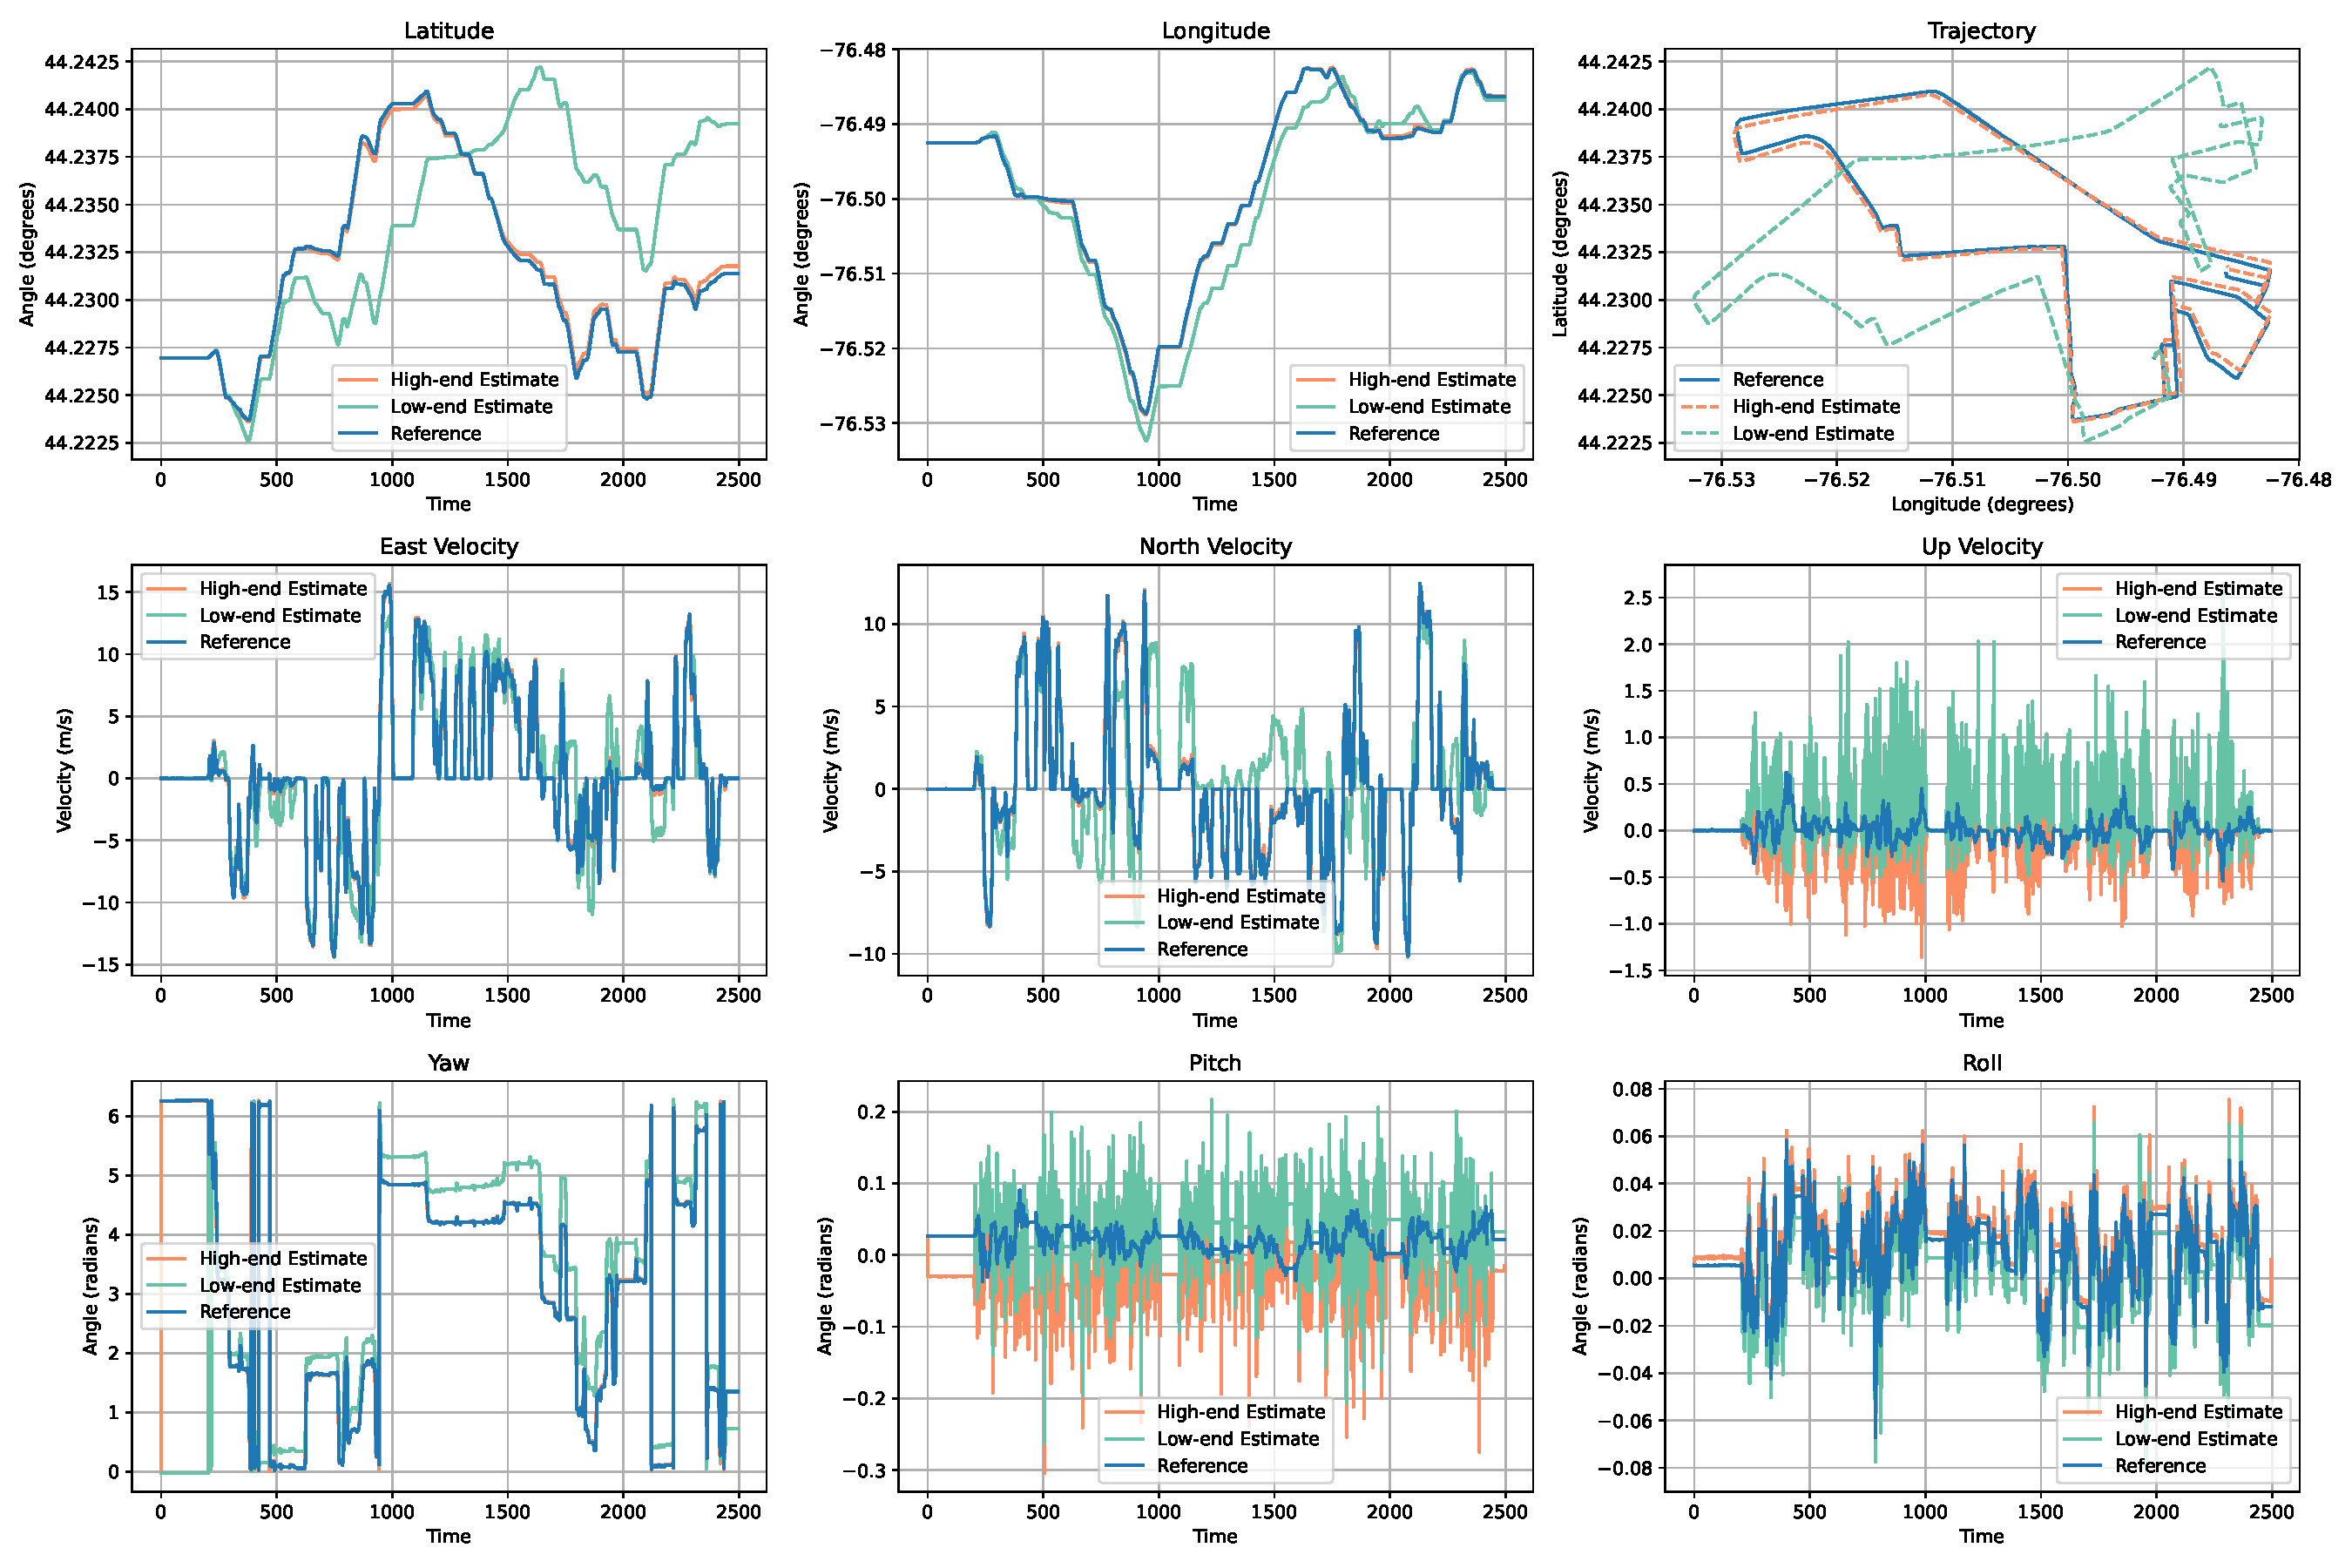
\includegraphics[width=1\textwidth]{plots/combined_plot.pdf}
    \caption{Plots of positional, velocity, and attitude components for high-end and low-end IMU data.}
    \label{fig:imu_data}
\end{figure*}

Figure~\ref{fig:imu_data} shows plots of the horizontal positional components (latitude and longitude), velocity components (east, north, and up), and attitude components (yaw, pitch, and roll) for both the high-end and low-end IMU data.

\begin{table*}[htbp]
\caption{Positional Error Metrics for High-End IMU Data}
\begin{center}
\begin{tabular}{|c|cc|cc|cc|cc|cc|}
\hline
\textbf{System Configuration} & \multicolumn{2}{c|}{$\delta P_E$} & \multicolumn{2}{c|}{$\delta P_N$} & \multicolumn{2}{c|}{$\delta h$} & \multicolumn{2}{c|}{$\delta P_{2D}$} & \multicolumn{2}{c|}{$\delta P_{3D}$} \\ \hline
                              & \textbf{RMS (m)} & \textbf{\%} & \textbf{RMS (m)} & \textbf{\%} & \textbf{RMS (m)} & \textbf{\%} & \textbf{RMS (m)} & \textbf{\%} & \textbf{RMS (m)} & \textbf{\%} \\ \hline
Baseline (INS core)           & 13.7            & 0.2\%       & 27.4            & 0.4\%       & 101.5           & 52.2\%      & 30.6            & 0.2\%       & 106             & 0.8\%       \\ \hline
INS + Bias Estimation         & 69.7            & 0.8\%       & 137.9           & 2.16\%      & 123.8           & 63.7\%      & 154.5           & 1.2\%       & 198             & 1.6\%       \\ \hline
INS + Stop Mechanization      & 118.2           & 1.3\%       & 203           & 3.2\%       & 101.5           & 52.2\%      & 235             & 1.8\%       & 256             & 2\%         \\ \hline
Full System                   & 97.1            & 1.0\%       & 204.1           & 3.2\%       & 123.8           & 63.7\%      & 226             & 1.8\%       & 258             & 2\%         \\ \hline
\end{tabular}
\label{table:high_end_errors}
\end{center}
\end{table*}

\begin{table*}[htbp]
\caption{Positional Error Metrics for Low-End IMU Data}
\begin{center}
\begin{tabular}{|c|cc|cc|cc|cc|cc|}
\hline
\textbf{System Configuration} & \multicolumn{2}{c|}{$\delta P_E$} & \multicolumn{2}{c|}{$\delta P_N$} & \multicolumn{2}{c|}{$\delta h$} & \multicolumn{2}{c|}{$\delta P_{2D}$} & \multicolumn{2}{c|}{$\delta P_{3D}$} \\ \hline
                              & \textbf{RMS (m)} & \textbf{\%} & \textbf{RMS (m)} & \textbf{\%} & \textbf{RMS (m)} & \textbf{\%} & \textbf{RMS (m)} & \textbf{\%} & \textbf{RMS (m)} & \textbf{\%} \\ \hline
Baseline (INS core)           & 1379           & 15.6\%      & 613.4           & 9.6\%       & 314.3           & 161.7\%     & 1509.4           & 12\%        & 1541.8           & 12.2\%      \\ \hline
INS + Bias Estimation         & 214.4           & 2.4\%       & 746.3           & 6.2\%       & 306.8           & 157\%       & 776.4           & 6.2\%       & 834.8           & 6.6\%       \\ \hline
INS + Stop Mechanization      & 746.6           & 8.4\%       & 752.9           & 11.8\%       & 314.3           & 161.7\%     & 1060.4           & 8.4\%       & 1105.9           & 8.7\%       \\ \hline
Full System                   & 255.2           & 2.9\%       & 671.5           & 10.5\%       & 306.8           & 157\%       & 718.3           & 5.7\%       & 781.1           & 6.2\%       \\ \hline
\end{tabular}
\label{table:low_end_errors}
\end{center}
\end{table*}


To assess the system’s performance, a reference trajectory was used, generated by integrating GPS data with the high-end tactical IMU. Positional errors were evaluated using root mean square (RMS) errors and errors expressed as a percentage of the distance traveled. The errors were calculated for the individual components (east, north, and altitude) as well as the overall horizontal 2D positional error and 3D positional error. Table~\ref{table:high_end_errors} summarizes the errors for the high-end IMU data, while Table~\ref{table:low_end_errors}  presents the corresponding errors for the low-end IMU data. These tables highlight the impact of estimating sensor biases and stopping mechanization when the vehicle is stationary. Filtering results are presented separately in Table~\ref{table:altitude_rms}.

\begin{table}[htbp]
\caption{RMS Altitude Errors (in meters) for High-End and Low-End IMU Data Using Different Filtering Techniques}
\begin{center}
\begin{tabular}{|c|c|c|}
\hline
\textbf{Filtering Technique} & \textbf{High-End Data (m)} & \textbf{Low-End Data (m)} \\ \hline
Baseline                      & 101.5                      & 306.8                     \\ \hline
MA ($N = 3$)                  & 21.1                       & 396.9                     \\ \hline
EMA ($\alpha = 0.4$)                & 20.6                       & 467.3                     \\ \hline
BW ($N = 2$, $f_c = 0.2$)       & 20.4                       & 402.9                     \\ \hline
\end{tabular}
\label{table:altitude_rms}
\end{center}
\end{table}


Additionally, Table~\ref{table:altitude_rms} provides
the RMS errors of the altitude component using different filtering techniques for both high-end and low-end IMU data. All the different filtering techniques were combined with Tustin's approximation of the derivative where $\beta = 0.1$. Figure~\ref{fig:altitude_comparison} demonstrates the effect of EMA filtering combined with Tustin’s approximation of the derivative on the altitude estimation.

\begin{figure*}[htbp]
    \centering
    \begin{minipage}{0.48\textwidth}
        \centering
        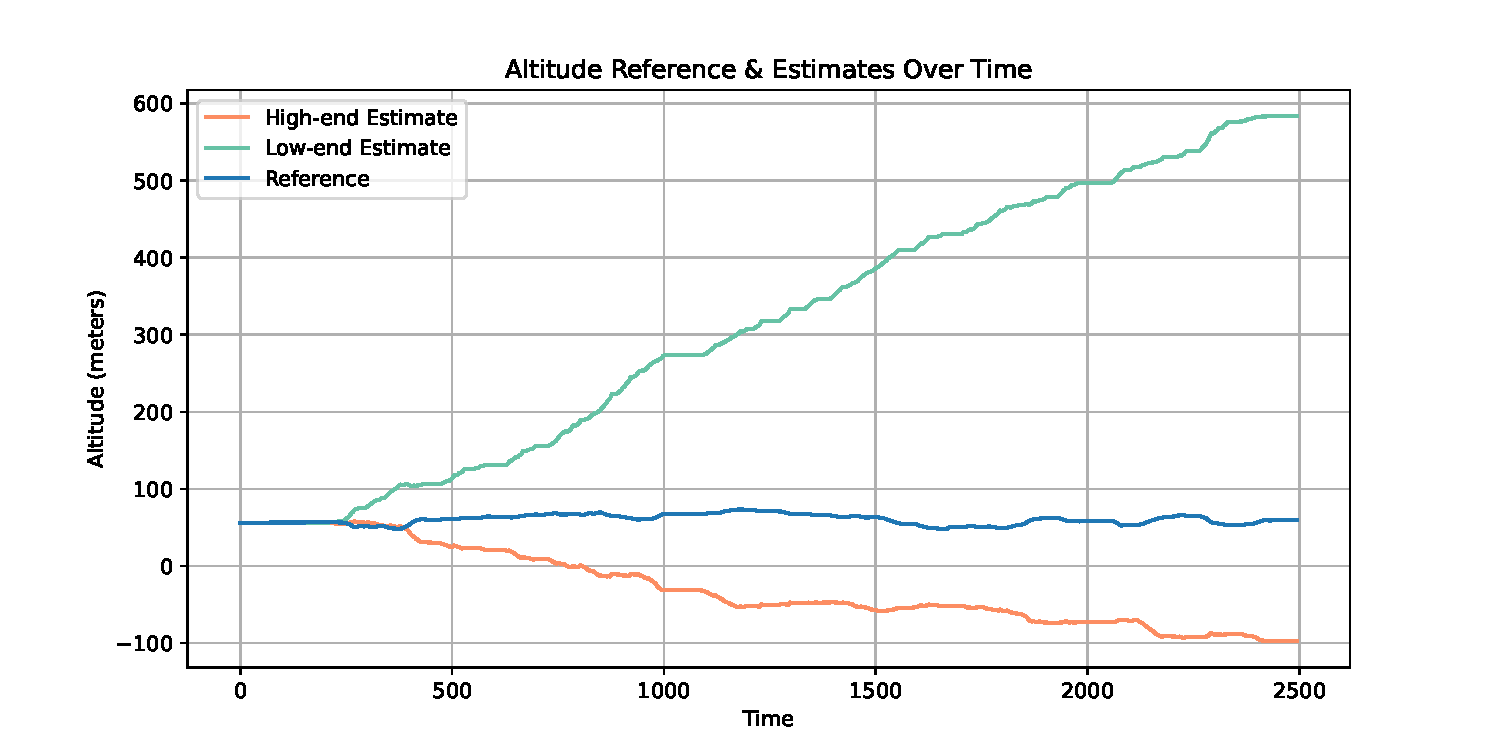
\includegraphics[width=\linewidth]{plots/alt.pdf}
        \caption*{(a) Altitude before filtering}
    \end{minipage}\hfill
    \begin{minipage}{0.48\textwidth}
        \centering
        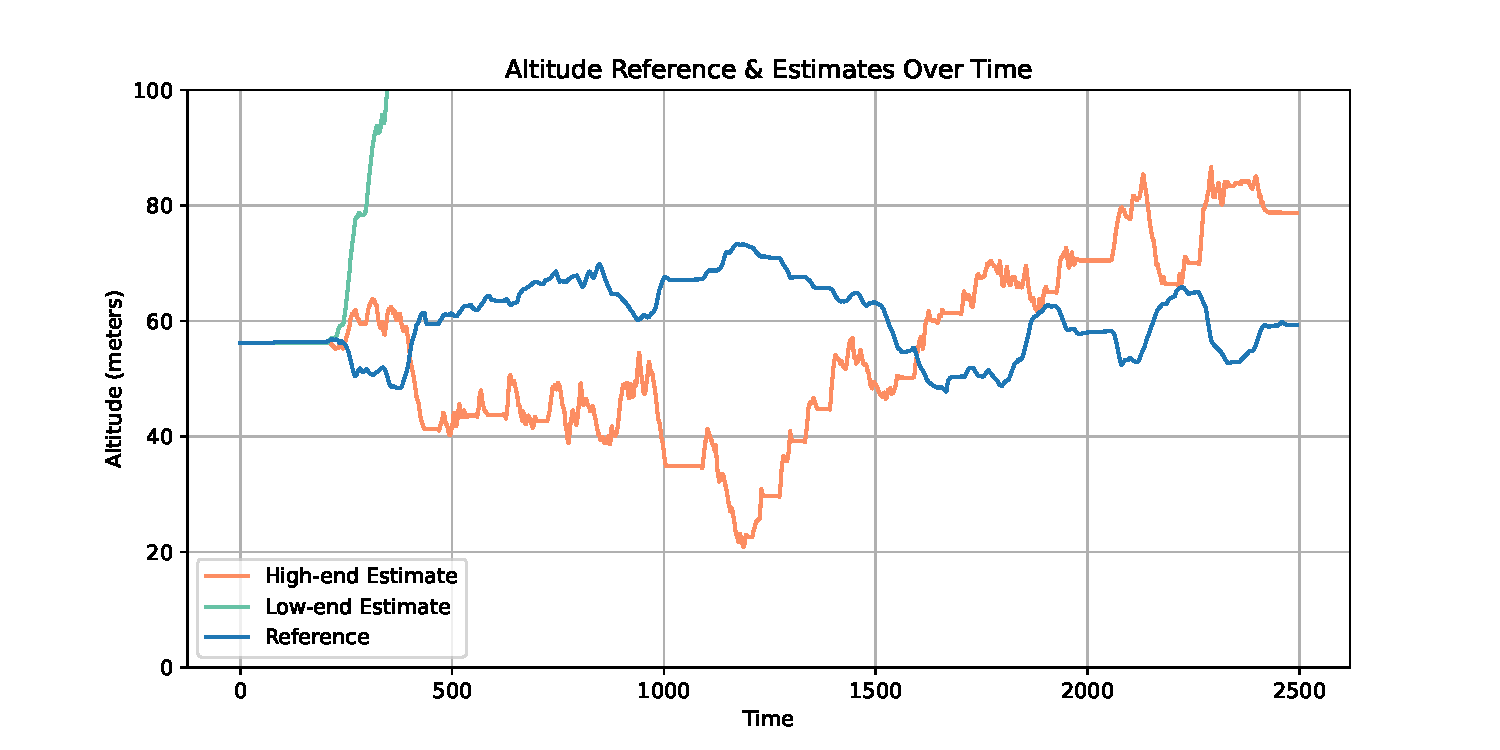
\includegraphics[width=\linewidth]{plots/alt_filt.pdf}
        \caption*{(b) Altitude after EMA filtering}
    \end{minipage}
    \caption{Altitude for high-end and low-end data before and after applying an EMA filter.}
    \label{fig:altitude_comparison}
\end{figure*}

\section{Discussion}

\subsection{Advantages \& Limitations of the 3-D RISS}

The proposed 3-D Reduced Inertial Sensor System (RISS) offers significant advantages over a full Inertial Measurement Unit (IMU) due to two primary factors: (1) the calculation of pitch and roll using accelerometers instead of gyroscopes and (2) the calculation of velocity based on the vehicle’s odometer-derived speed instead of accelerometers. These improvements reduce the accumulation of errors and enhance navigation system performance.

One of the key improvements in the RISS system is the use of accelerometers for calculating pitch and roll instead of gyroscopes. In traditional IMUs, an uncompensated bias $b_w$ in one of the horizontal gyroscopes leads to angle errors that grow proportionally with time, $\delta \theta_1 = \int b_w \, dt = b_w t$. This angle error introduces a misalignment in the Inertial Navigation System (INS) when projecting acceleration from the body frame to the local-level frame. The resulting misalignment causes errors in acceleration, velocity, and position, which are expressed as follows:
\begin{itemize}
    \item \textbf{Acceleration error:} $\delta a_1 = g \sin(\delta \theta) \approx g b_w t$
    \item \textbf{Velocity error:} $\delta v_1 = \int b_w g t \, dt = \frac{1}{2} b_w g t^2$
    \item \textbf{Position error:} $\delta p_1 = \int \delta v_1 \, dt = \frac{1}{6} b_w g t^3$
\end{itemize}

The gyroscope bias introduces a third-order error in position ($t^3$), which has a significant impact on navigation accuracy. By using accelerometers to calculate pitch and roll, the first integration is eliminated, reducing the cumulative error growth rate from $t^3$ to $t^2$. This makes the system more resilient to drift and improves its overall performance.

The second advantage of the RISS system lies in its calculation of velocity using the vehicle’s odometer-derived speed rather than accelerometers. In conventional systems, an uncompensated accelerometer bias $b_f$ introduces errors that propagate as follows:
\begin{itemize}
    \item \textbf{Velocity error:} $\delta v_2 = \int b_f \, dt = b_f t$
    \item \textbf{Position error:} $\delta p_2 = \int \delta v_2 \, dt = \frac{1}{2} b_f t^2$
\end{itemize}

By relying on the odometer for velocity calculation, the first integration step is eliminated, resulting in fewer accumulated errors and more accurate position estimation. In addition, the bias and scale factors of odometers are more stable than that of accelerometers.

The main limitation of the 3-D RISS lies in differentiating velocity readings to estimate pitch and roll, as differentiation is mathematically equivalent to applying a high-pass filter, which inherently introduces a significant amount of noise. This noise can degrade the accuracy of downstream estimates. Since pitch and roll estimates play a critical role in 3D alignment from the vehicle’s body frame to the local-level frame, yaw and velocity components are directly affected, and by effect the propagation of errors affects position estimates.

\subsection{Observations and Insights}

The tabulated positional errors highlight the superior performance of the high-end IMU system compared to the low-end system. This can be attributed to the significantly better performance specifications of the high-end unit, such as lower bias instability, reduced bias drift over temperature, minimal scale factor non-linearity, and lower angle random walk. These characteristics ensure that the high-end IMU provides more accurate and stable measurements of angular velocity and linear acceleration over time, leading to better integration for position estimation. In contrast, low-end IMUs, with poorer bias stability and higher noise levels, introduce larger accumulated errors due to sensor drift and noise amplification during integration. As a result, navigation performance in low-cost systems is more prone to degradation, particularly during long-duration operations where uncompensated errors accumulate rapidly, leading to increased positional and altitude errors.

Upon inspecting the plots of yaw estimates from both IMU units against the reference trajectory, significant deviations are observed during sharp changes in the yaw angle, typically occurring during sharp turns. These deviations are critical, as they directly impact the horizontal positional components, specifically latitude and longitude. The reason for this lies in the role of yaw estimates in aligning the vehicle’s forward velocity \( v_{od} \) with the local-level frame. Incorrect yaw estimates result in errors when projecting \( v_{od} \) into the east and north velocity components, which are then integrated to determine latitude and longitude. As a result, even small errors in yaw during dynamic maneuvers can propagate into substantial horizontal positional errors over time, degrading the overall navigation performance.

\subsection{Analysis of Performance Degradation in High-End IMU with Bias Correction and Stationary Detection}

The observed improvement in the performance of the low-end Inertial Measurement Unit (IMU) after implementing bias correction and stationary detection, contrasted with the degradation in high-end IMU performance, may be attributed to differences in sensor noise characteristics, bias stability, and the impact of dead reckoning interruptions.

High-end IMUs typically have low noise and highly stable biases, meaning their raw measurements are already accurate over long periods. If the true bias of a high-end sensor is small and stable over time, then any attempt to estimate it over a short time window (like during initialization) may overestimate or misrepresent the actual bias. In contrast, low-end IMUs often experience significant and time-varying biases, making even approximate corrections beneficial by reducing cumulative errors.

Stopping the dead reckoning loop during stationary periods was beneficial for the low-end IMU because it prevented the integration of noisy sensor data, which would otherwise lead to rapid error accumulation. However, for the high-end IMU, this interruption may have disrupted its natural advantage of maintaining stable, time-correlated errors. Continuous estimation allows high-end IMUs to exploit this correlation, keeping errors bounded. By stopping the loop and reinitializing after stationary periods, small initialization errors—particularly in velocity and heading—could have compounded over time, degrading overall accuracy.

This explanation suggests that the performance differences arise because corrections and dead reckoning interruptions effectively mitigate the large, random errors of low-end IMUs but interfere with the stable estimation process of high-end IMUs.

\subsection{Altitude Estimation: Divergence and Mitigation Approaches}

The divergence in the altitude estimate for both high-end and low-end IMU data Figure~\ref{fig:altitude_comparison} was primarily driven by bias errors in the accelerometers and noise introduced during the differentiation operation used to estimate the pitch angle. These errors propagated through the upward velocity calculation and, when integrated over time, led to numerical instability and cumulative drift in the altitude estimate. To mitigate this issue, an exponential moving average (EMA) filter was selected due to its ability to significantly reduce noise while maintaining an extremely low computational cost of \( O(1) \). The EMA was coupled with Tustin’s approximation of the derivative, using a parameter \( \beta = 0.1 \), to stabilize the estimation of the acceleration derived from odometer readings.

The tabulated results Table~\ref{table:altitude_rms} show that applying this combination improved the root-mean-square (RMS) error of the altitude by a factor of five for the high-end IMU and successfully prevented the altitude estimate from diverging. However, for the low-end IMU, the altitude estimate worsened and diverged further. This behavior can be explained by the low-end IMU’s higher sensor noise and larger, time-varying biases. While Tustin’s approximation and the EMA effectively suppressed small noise in the high-end IMU, they struggled to handle the large, rapidly fluctuating errors in the low-end IMU. The differentiation operation amplified these fluctuations, and the EMA filter, instead of smoothing them effectively, introduced lag and suppressed critical dynamic information. As a result, the pitch angle estimation became increasingly inaccurate, leading to incorrect upward velocity estimates and faster divergence of the altitude in the low-end case.

\section{Conclusion}

In conclusion, the proposed 3D Reduced Inertial Sensor System (RISS) demonstrates significant potential as a cost-effective navigation solution, especially for low-cost autonomous systems. By strategically reducing the reliance on multiple gyroscopes and leveraging accelerometer-based pitch and roll estimation, the system effectively addresses common issues related to bias drift and noise accumulation. The integration of heuristic-based enhancements, such as bias estimation and stationary detection, further improves its accuracy and stability.

The experimental results show that the high-end IMU consistently outperforms its low-end counterpart due to superior performance specifications, including lower bias instability and minimal noise amplification. However, the improvements achieved through bias correction and stopping mechanization during stationarity proved especially beneficial for low-end systems, significantly reducing cumulative errors.

Despite these advances, the system’s performance during dynamic maneuvers, such as sharp turns, highlights areas for further improvement. Errors in yaw estimation propagate into horizontal position inaccuracies, and noise in pitch and roll estimation affects altitude stability. The application of advanced filtering techniques, such as the exponential moving average (EMA) combined with Tustin’s approximation, demonstrated success in mitigating these issues for high-end data. However, the low-end IMU remained susceptible to noise amplification and divergence, pointing to the need for further refinement in handling low-cost sensor limitations.

Overall, this work illustrates that a carefully designed RISS can provide robust and reliable navigation in resource-constrained applications, with promising avenues for future optimization focused on noise suppression and dynamic correction mechanisms tailored for low-end systems.

%\section*{References}

\begin{thebibliography}{00}

\bibitem{noureldin2013} A. Noureldin, T. B. Karamat, and J. Georgy, \textit{Fundamentals of Inertial Navigation, Satellite-Based Positioning and Their Integration}. Berlin, Germany: Springer-Verlag, 2013.
\bibitem{ogata2010} K. Ogata, \textit{Discrete-Time Control Systems}, 2nd ed. Upper Saddle River, NJ, USA: Prentice Hall, 2010.
\bibitem{manolakis2011} D. G. Manolakis and V. K. Ingle, \textit{Applied Digital Signal Processing: Theory and Practice}. Cambridge, U.K.: Cambridge University Press, 2011.



\end{thebibliography}

\end{document}
